% Chapter Template

\chapter{ Self-Growing Recurrent Neural Network} % Main chapter title

\label{Chapter 2} % Change X to a consecutive number; for referencing this chapter elsewhere, use \ref{ChapterX}

\lhead{Chapter 2. \emph{Self-Growing Recurrent Neural Network}} % Change X to a consecutive number; this is for the header on each page - perhaps a shortened title

%----------------------------------------------------------------------------------------
%	SECTION 1
%----------------------------------------------------------------------------------------

%\section{State of the Art}

\section{Motivation}

In this Chapter, we introduce Self-Growing Recurrent Neural Network (SGRNN), which is a Recurrent Neural Network that change its architecture as well as its weights during learning. In the standard Recurrent Neural Network, the hidden-to-hidden weight Matrix ($W_{hh}$) is considered as a dense Matrix in the calculation. This means that each neuron is connected to all the other neurons and that each weight takes the same ammount of computation time to update. Therefore, the learning step in the hessian free optimization (HFO) or stochastic gradient descent compute an update for each elements of this weight matrix. However, from a biological perspective, it makes sense to restrict the connections of a neuron to neuron that are near it. Performing such a change in the architecture of a RNN, reduce the number of connections complexity from $O(n^2)$ to $O(n)$. The same observation can be made for inputs and outputs weights as each neuron in the RNN neuron have inputs and outputs weights. Such an architecture change could reduce the computation time as well as the memory usage for the same number of neurons using sparse matrix representation. 

Another important part of learning for a human being is the brains plasticity. The brain has the abbility to add and destroy neurons and connections when it is developping. Especially during childhood. SGRNN propose a new step in the learning process to model this phenomena : the capacity to add and remove neurons during training.

\section{SGRNN}

The SGRNN structure is the same as the standard RNN. The difference come from the learning algorithm. The goal is to introduce a modification of the architecture during learning. Every $k$ steps of a Hessian Free Optimization or Stochastic Gradient Descent ( which are the state of the art method used to train RNNs) we perform this modification. Such a modification has to keep the global functioning of the RNN so that the previous learning steps are not useless. Based on the previous chapter experiments, we propose an empirical solution in performing such a step called the \verb?evolutionStep? in Algorithm 1. The goal of this step is to delete neurons and connections which have a small or no contribution to the model and duplicate neurons (and connections) where it seems important.   
$$
\begin{array}{rcr} 
    h_0 & = & a(W_{hx}  * x_0 + b_{init} + b_h)  \\ 
    h_i & = & a(W_{hx}  * x_i + W _{hh} * h_{i-1} + b_h)  \\ 
    \hat{y}_i & = & a'(W_{yh} + b_y)

\end{array}
$$


\begin{algorithm}
    \caption{Learning algorithm}
    \begin{algorithmic}
    \STATE $ weightsInit() $
    \WHILE{$continueTraining$}
        \FOR{$i \in [1: K]$}
            \STATE $HFOStep()$
        \ENDFOR
        \STATE $evolutionStep()$
    \ENDWHILE
    
    \end{algorithmic}
\end{algorithm}

\subsection{Implementation of the Hessian Free Optimization step}
The Hessian Free Optimization \cite{martens2011learning} is implemented using the Theano library, that handle efficient symbolic differentiation (on GPU), especially for multi-dimensional arays, which makes it the perfect candidate to test and implement new models of Recurrent Neural Networks. Boulanger \cite{boulanger2012modeling} implemented the Hessian-Free optimization method with Martens \& Sutskever \cite{martens2011learning} improvements. 

Theano handles the differenciation automaticly once provided an expression such as the one defining RNNs. It is then possible to use the gradient function to obtain the gradient of this expression with respect to a list of parameters.

However the SGRNN step requires only to compute the gradient over the non-zero values in the sparse matrix representation of the hidden-to-hidden weight matrix. Therefore, we provide a mask to the RNN implementation, and we replace $W_{hh}$ with the hadamard product $M \circ  Whh$ , where $M$ is the mask, ie a binarry matrix that contains $1$ where there is a connection between neurons and $0$ elsewhere. Using this trick it is possible to use the classical Hessian free optimization (or a stochastic gradient descent) as the gradient of the network in respect to $Whh_{ij}$ is guaranted to be null if there is no connection between neuron $i$ and $j$. However this implementation does not bring speed nor memory improvements of the HFO step and therfore was not used in the following experiments on SGRNN(see Future Work).


\subsection{Weights Initialization}

    In a standard RNN, the weight matrices are randomly initialized, in order to prevent symmetry that could not be broken during the learning phase within the model. The same initialization techniques are used. However, a smaller number of neurons is required as new neurons will be introduced during training.  

\subsection{Evolution Step}

The evolution step consist of two different steps that we named using the Gentic Algorithm conventions as they have a similar meaning. 
\begin{itemize}
    \item A selection step, where we delete connections and Neurons.
    \item A cross-over step, where we introduce new neurons and connections. 
\end{itemize}

\subsubsection{Selection}

In order to perform the selection step we need an estimation of the worth of neuron or a connection. Based on the experiments in the previous chapter, we saw that none of the metrics that seemed natural to judge the worth of a neuron or a connection (for example the sum of the absolute value of the weights ) provide satisfying results. Therefor in this project we used the same approach that was used as the benchmark to judge the worth of a neuron in the previous chapter: We delete the neuron and mesure the performance of the network on a validation set. 

\subsubsection{Cross-Over}

In order to introduce new neurons without, "breaking" all the networks dynamic and having to start learning from the start, we use a technique to duplicate neurons. We construct new neurons that we clone from an existing neuron. We then create a neuron that will have the same state with a small noise when cloned. This is done using the same input connections as the cloned neuron, and dividing by 2 all output connections. We also introduce a small noise on the Whh matrix for the new neurons so that it is not exactly the same. (Otherwise the HFO step will not make use of the new parameters as they will have exactly the same gradient informations.) The following code sample explains the performed operations : For $Whh$, a copy of the column containing the neuron to clone is added to the matrix (this correspond to the inputs of the hidden connections), the row containin the neuron to clone is first multiplied by $0.5$ and then added to the matrix. The \verb?noise? use a mutivariate normal distribution sample using as mean the row $v$ (or column) and as covariance matrix a diagonal matrix that contains $0.01 * v$. For $Whx$ only the column is added (input)and for $Why$ half the row in the same way as $Whh$. For the biases vectors, h0 and bh contain 1 more element : the bias of the cloned neurons. 

\begin{verbatim}

def noise(self, vector):
    #return vector
    cov = 0.01 * np.diag(np.abs(vector))
    res = np.random.multivariate_normal(vector, cov)
    return res.astype(theano.config.floatX)

def insert_in_model(self, i):
    #clone neurons i
    self.whh = np.array(np.hstack([self.whh, np.matrix(self.noise(self.whh[:, i])).T])) 
    self.whh[i] = 0.5 * self.whh[i]  
    self.whh = np.vstack([self.whh, self.noise(self.whh[i])])  # TODO add noise

    self.mask = np.vstack([self.mask, self.mask[i]])
    self.mask = np.array(np.hstack([self.mask, np.matrix(self.mask[:, i]).T]))

    self.Wx = np.array(np.hstack([self.Wx, np.matrix(self.Wx[:, i]).T])) 
    self.bh = np.hstack([self.bh, self.bh[i]]) 
    self.h0 = np.hstack([self.h0, self.h0[i]])

    self.Wy[:, i] = 0.5 * self.Wy[:, i]  
    self.Wy = np.array(np.vstack([self.Wy, self.Wy[i]])) 

    self.p = [self.Wx, self.whh, self.Wy, self.bh, self.by, self.h0]

\end{verbatim}

Without the noise, this would make the network equivalent to the previous one. Therefore, as long as the noise does not affect the dynamic of the network to much, the new network is pre-trained with the smaller network.

Using this technique we can easily introduce new neurons in the network.

Finding neurons/connections based on the performance of the network on a validation set witout them provide a choice for deleting neurons. However, finding the neurons that are fitted to be duplicated is trickier as we have no direct way of ordering the neurons for this. Therefore in this project we made the following assumption : The neurons that are the most necessary to the network are the best candidate to be duplicated. We discuss the validity of this assumption in the conlusion and Future work chapter.  


\section{Experiment}

We tested the SGRNN on a dataset of Music files in the MIDI format. Using code sample from \cite{boulanger2012modeling} to parse Midi files, we convert the files into a vector of bits, 1 for each timestep (sampling every 0.3 sec), where notes from the piano keyboard are numeroted (from $0$ to $88$ ) and $0$ corresponds to the fact that the note is not "on" for this timestep and $1$ that the note is currently "on". Using this representation method it is then possible to feed this sequencial data to a RNN. During training we tested with $10$ timesteps-long sequences, to produce a large enough dataset of sequence (though for this particular problem, it seems more suited to experiment with longer sequences) The network is asked on the 9-th timestep to predict the entry of the 10th. By using this technique we train the network to predict what are the possible following of a sequence. As the prediction is a vector of float within $[0, 1]$ we use the cross-correlation error in the Hessian Free optimization 
$$ (-t* T.log(y) - (1-t)* T.log(1-y)).mean() $$

We also mesure the prediction error on the training set as well as a validation set, by compairing the value of ($o>0.5$) and the corresponding bit for every prediction of the newwork.

The network is trained to predict the next element after a sequence and therefore we can use it to generate sequences. We initialize the network with a random sequence or a sequence from the test set and let it predict the next element. Then we shift all values in the sequence from 1 and place the precedent predicted value as the last element, and thatway we predict a new element. We then shift the sequence again and place the second value to the end. By repeting this steps many times, we can generate music. 


    
\begin{figure}[htbp]
    \centering
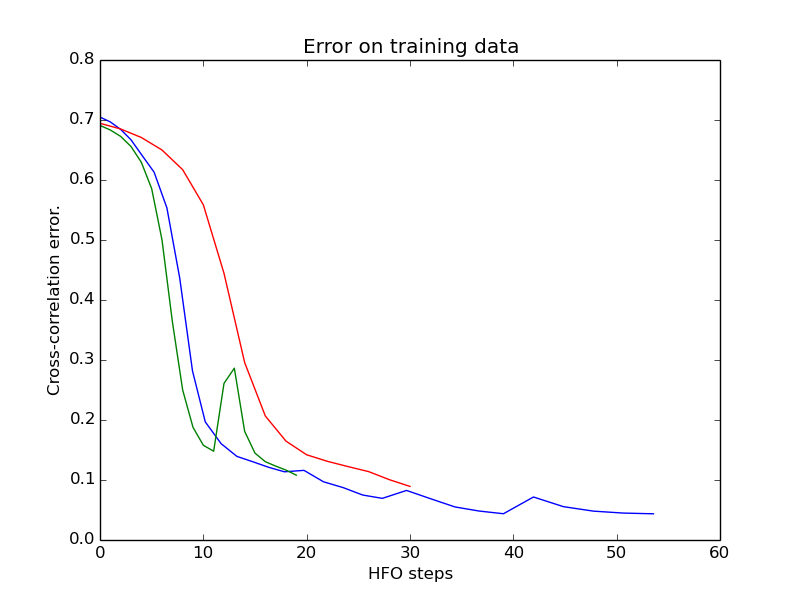
\includegraphics[scale=0.7]{Figures/sgrnn_training.png}
    \rule{35em}{0.5pt}
    \caption[Learning curves]{Learning curves}
    \label{fig:init_roll}
\end{figure}

In figure \ref{fig:init_roll} we plot the cross-correlation error on a validation set after each HFO step. In green we ploted the learning curve for a RNN with 20 neurons, and in red for a RNN with 40 neurons. The blue curve is the learning curve of the SGRNN initiated with $20$ neurons, and using a selection ratio of $75$ percent and a cross-over ratio of $165$ percent. We can observe the evolution steps on the end of the blue learning curve, as evolution steps induce a larger error ( because of the noise and the deleted neurons) in the end. We also generated a sample before learning and at the end of learning. The sample are displayed on \ref{fig:init_roll} and \ref{fig:piano_roll} where for each timet-step we plot in black the number corresponding to notes that are "on" and can also be recorded.


    
\begin{figure}[htbp]
    \centering
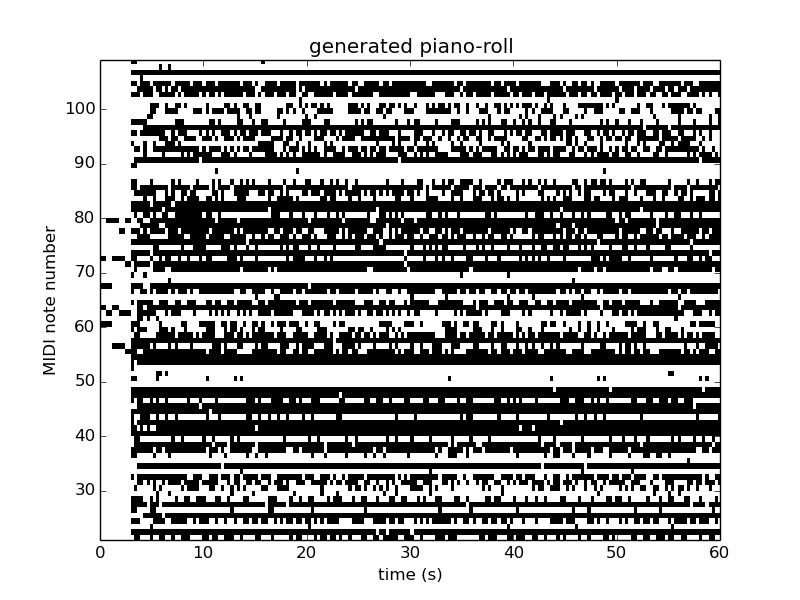
\includegraphics[scale=0.5]{Figures/init_piano_roll.png}
    \rule{35em}{0.5pt}
    \caption[Generated music at initialization of the RNN]{Generated music at initialization of the RNN}
    \label{fig:init_roll}
\end{figure}


\begin{figure}[htbp]
    \centering
    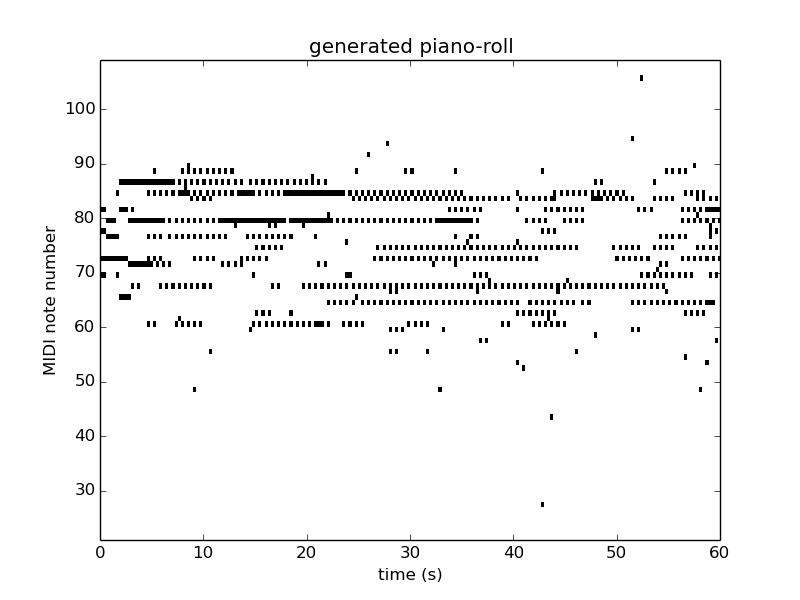
\includegraphics[scale=0.5]{Figures/piano_roll.png}
    \rule{35em}{0.5pt}
    \caption[Generated music after training]{Generated music after training}
    \label{fig:piano_roll}
\end{figure}


